\documentclass[12pt]{article}
\usepackage{amsmath}
\usepackage{light}
\usepackage{graphicx}

\hidesolutions

\newcommand{\mfigure}[3]{\bigskip\centerline{\resizebox{#1}{#2}{\includegraphics{#3}}}\bigskip}
\newcommand{\naturals}{\mathbb N}
\newcommand{\eqdef}{:=}
\newcommand{\prsub}[2]{\mathop{\textup{Pr}_{#1}}\nolimits\left(#2\right)}

\newcommand{\edge}[2]{#1\text{---}#2}

\newcommand{\todo}[1]{\emph{TODO: #1}}
\newcommand{\remark}[1]{\emph{#1}}
\newcommand{\skipthis}[1]{}



\newcommand{\quizz}[2]{
    \vspace*{-2cm}
  \noindent \coursename \hfill #2 \newline
  \coursestaff \vspace{-1.5ex} \newline
  \mbox{} \hrulefill \mbox{}
%  \vspace{-0.15in}
  \begin{center}
    \ifthenelse{\boolean{showsolutions}}
               {\Large \textbf{Quiz #1 Solutions}}
               {\Large \textbf{Quiz #1}}
  \end{center}
  \vspace{-.1in}
  \thispagestyle{plain}
  \pagestyle{myheadings}
  \thispagestyle{empty}
  \markboth{Quiz #1}{Quiz #1}
  %\coursecopyright
  }

\begin{document}

\quizz{2}{11/13/2012}


\begin{itemize}

\item  The quiz is \textbf{closed book}, but you may have two $8.5''  \times 11''$ sheet with notes (either printed or in your own handwriting) on both sides.

\item Calculators and electronic devices (including cell phones) are not allowed.

\item You may assume all of the results presented in class. This does \textbf{not} include results demonstrated in practice quiz material.

 \item Please show your work. Partial credit cannot be given for a wrong answer if your work isn't shown.

 \item Write your solutions in the space provided. If you need more space, write on the back of the sheet containing the problem. Please keep your entire answer to a problem on that problem's page.

 \item Be neat and write legibly. You will be graded not only on the correctness of your answers, but also on the clarity with which you express them.

 \item  If you get stuck on a problem, move on to others. The problems are not arranged in order of difficulty.\\


 \textbf{NAME:} \rule{5in}{0.5pt}\\
 
 \textbf{TA:} \rule{5.34in}{0.5pt}\\
 
\centering
\scalebox{1.5}{
\begin{tabular}{|c|c|c|c|}
\hline
\textbf{Problem} & \textbf{Value} & \textbf{Score} & \textbf{Grader} \\\hline
1 & 11 & & \\\hline
2 & 10 & & \\\hline
3 & 10 & & \\\hline
4 & 10 & & \\\hline
5 & 8 & & \\\hline
6 & 10 & & \\\hline
7 & 12 & & \\\hline
8 & 7 & & \\\hline
%10 & 10 & & \\\hline
9 & 12 & & \\ \hline
10 & 10 & & \\ \hline
\textbf{Total} & 100 & & \\\hline
\end{tabular}
}
\end{itemize}

\newpage

\begin{problem}{11}

 %   \remark{Maybe find a more interesting partial order to use instead.}

Fix positive integers $k$ and $n$ with $k \leq n$. Let 
\[ \mathcal{X} = \{ S \subseteq \{1, 2, \ldots, n\} \,:\, |S| \leq k \}. \]
Consider the following relation from $\mathcal{X}$ to $\mathcal{X}$:
\[ R = \{ (S,T) \in \mathcal{X} \times \mathcal{X} \,:\, S \subseteq T \}. \]

\bparts
\ppart{7} Prove that $R$ is a (weak) partial order on $\mathcal{X}$.
\vspace{8cm}

\newpage

\ppart{4} Take $n=4$ and $k=2$. Draw the Hasse diagram of the partial order.
\eparts

\end{problem}

\newpage

\begin{problem}{10}
\bparts

\newcommand{\longline}{\underline{\hspace{5cm}}}

\ppart {5}
Order the following functions from 1 through 6 so that your $i$\textsuperscript{th} choice is $\emph{big-O}$ of your $(i+1)$\textsuperscript{th} choice (so the function you mark $1$ should be smallest, and 6 largest).
%Arrange the functions $n^n$, $(\log n)^2$, $n^{1.0001}$, $(1.0001)^n$, $2^{\sqrt{\log_2n}}$, and, $n(\log n)^{1001}$ in a list so that each function is \emph{big-O} of the next-function. 

\bigskip

\renewcommand{\arraystretch}{3}
\begin{tabular}{ll}
    $n^n$ & \longline \\
$(\log n)^2$ & \longline \\
$n^{1.0001}$ & \longline \\
$(1.0001)^n$ & \longline \\
$2^{\sqrt{\log_2n}}$ & \longline \\
 $n(\log n)^{1001}$  & \longline \\
\end{tabular}
\renewcommand{\arraystretch}{1}

\newpage

\ppart{5} Identify and explain the mistake in
the ``proof'' of the following bogus claim.
\begin{falseclm*}
\begin{equation}\label{2n1}
2^n = O(1).
\end{equation}
\end{falseclm*}

\begin{proof}
The proof is by induction on $n$ where the induction 
hypothesis, $P(n)$, is the assertion~\eqref{2n1}.

{\bf Base case:}  $P(0)$ holds trivially.

{\bf Inductive step:} Assume $P(n)$ to prove $P(n+1)$. So there is a constant $c >0$
such that $2^n \leq c \cdot 1$.  Therefore,
\[
2^{n+1} = 2 \cdot 2^n \leq (2c) \cdot 1,
\]
which implies that $2^{n+1} = O(1)$.  That is, $P(n+1)$ holds, which
completes the proof of the inductive step.

We conclude by induction that $2^n = O(1)$ for all $n$.  
%That is, the exponential function is bounded by a constant.
\end{proof}
\eparts

%\solution{.}
\end{problem}

\newpage

\begin{problem}{10}
    \bparts
    \ppart{3}
%Without appealing to Stirling's formula, 
Prove that
\[ \log (n!) = \Theta(n\log n). \]
\newpage

\ppart{7} Show that
\[ \sum_{k=1}^n 1/\log (k!) = \Theta(\log \log n). \]

\eparts
%\solution{.}
\end{problem}

%\emph{OR:} 
%\begin{problem}{10}
%
%Without appealing to Stirling's formula, prove that
%\[ \sum_{k=1}^n 1/\log (k!) = \Theta(\log \log n). \]
%
%\remark{Could split into two parts: first show $\log (n!) = \Theta (n \log n)$, and then the given question.}

%\end{problem}

\newpage
\begin{problem}{10}

Give a closed-form solution to the following recurrence
relation:
\[ G_n = 6G_{n-1} - 9G_{n-2} + 4n \quad \text{ for } n \geq 2, \qquad G_0 = 2,\; G_1 = 7. \]

%\solution{.}
\end{problem}


\newpage

\begin{problem}{8}
Find a $\Theta$ bound for the solution to the following recurrence:
    \begin{displaymath}
T(n) = 
\begin{cases}
1 & \text{if $n \leq 4$}\\
2T\left(\floor{{n\over 4}+ \sqrt{n}}\right)+\sqrt{n}
&  \text{if $n > 4$}\\
\end{cases}
\end{displaymath}

\solution{
We use the Akra-Bazzi formula. $p$ is the solution to
$2 \left({1 \over 4}\right)^p =  1$, so 
$p = 1/2$

\begin{eqnarray*}
\Theta \left( n^{1/2} + n^{1/2} \int_1^n {\sqrt{x} \over x^{3/2}} \right)
 & =  & \Theta \left( n^{1/2} + n^{1/2} \int_1^n {1 \over x} \right)\\
& = & \Theta ( n^{1/2} +  n^{1/2}\ln n)\\
& = & \Theta (n^{1/2}\ln n) 
\end{eqnarray*}
}

\end{problem}

\newpage


\begin{problem}{10}
Recall that the Fibonacci numbers are defined by
\[ F_1 = F_2 = 1, \qquad    F_n = F_{n-1} + F_{n-2} \; \text{ for } n \geq 3. \]
Prove, by induction, that
\[ F_{n+1}F_{n-1} = (F_n)^2 + (-1)^n \qquad \text{for all } n \geq 1. \]
\end{problem}

\newpage


\begin{problem}{12}

In a famous scene from the movie \emph{Ocean's Eleven}, Brad Pitt's character Rusty is teaching poker to some serious beginners. 
Shane West (playing himself) accidentally finds himself with a hand consisting of three pairs, which draws the remark from Rusty, ``You can't have three pairs. You can't have 6 cards in a 5-card game.''

Let's consider the fictional game of $6$-card poker, played from a standard deck of $52$ cards of 4 suits ($\clubsuit, \diamondsuit, \heartsuit, \spadesuit$) and $13$ ranks (1-10, J, Q, K, A).

\emph{Your solutions to the following questions may be in terms of combinatorial quantities like factorials and ${n \choose k}$. However, it may help you in double-checking your answer to know that three pairs should come out to be rarer than a full house.}

\bparts
\ppart{6} How many ``three-pairs'' hands are there? This is a hand with 2 cards of one rank, 2 cards of a second (different) rank, and 2 cards of a third (different) rank, for example, $3\heartsuit\; 3\diamondsuit\;5\clubsuit\; 5\heartsuit\;  J\spadesuit\; J\heartsuit$.

\newpage

\ppart{6} How many full house hands are there? This is a hand consisting of 3 cards of one rank, 2 cards of another (different) rank, and one single card of a third (different) rank: for example, $6\heartsuit\; 6\clubsuit\; 6\diamondsuit\; Q\diamondsuit\; Q\spadesuit\; A\heartsuit$ is a full house.


\vspace{6cm}

\solution{ 

We can create a bijection for three-pairs consisting of 3 ranks and 2 suits for each rank. This comes out to ${13 \choose 3}{4 \choose 2}^3 = 61,776$.

We can create a bijection for full house consisting of 1 rank with 3 suits, a second rank with 2 suits, and a third rank of any suit. This comes out to ${13 \choose 1}{4 \choose 3}{12 \choose 1}{4 \choose 2}{11 \choose 1}{4 \choose 1} = 164,736$, which is (much) larger than 61,776.}

\eparts
\end{problem}

\newpage


\begin{problem}{7}
%    \ppart{10}
    %Prove that any subset $C$ of $\{100, 101, 102, \ldots, 199\}$ with $|C|=51$ contains two consecutive integers.
    Prove that any subset $C$ of $\{101, 102, \ldots, 199, 200\}$ with $|C|=51$ contains two numbers that sum to $301$.

    \vspace{6cm}

%    \ppart{10} Alyssa P. Hacker is training for a marathon. Over a 20 day period, she will train 30 different times, but she will train at least once a day. Show that there is a period of consecutive days during which Alyssa trains \emph{exactly} 9 times. 
%
   % \remark{This one seems quite difficult.}

\end{problem}

\newpage

\begin{problem}{12}
    Consider an $n \times n$ chessboard (in the figure below, $n=8$).

    \begin{center}
        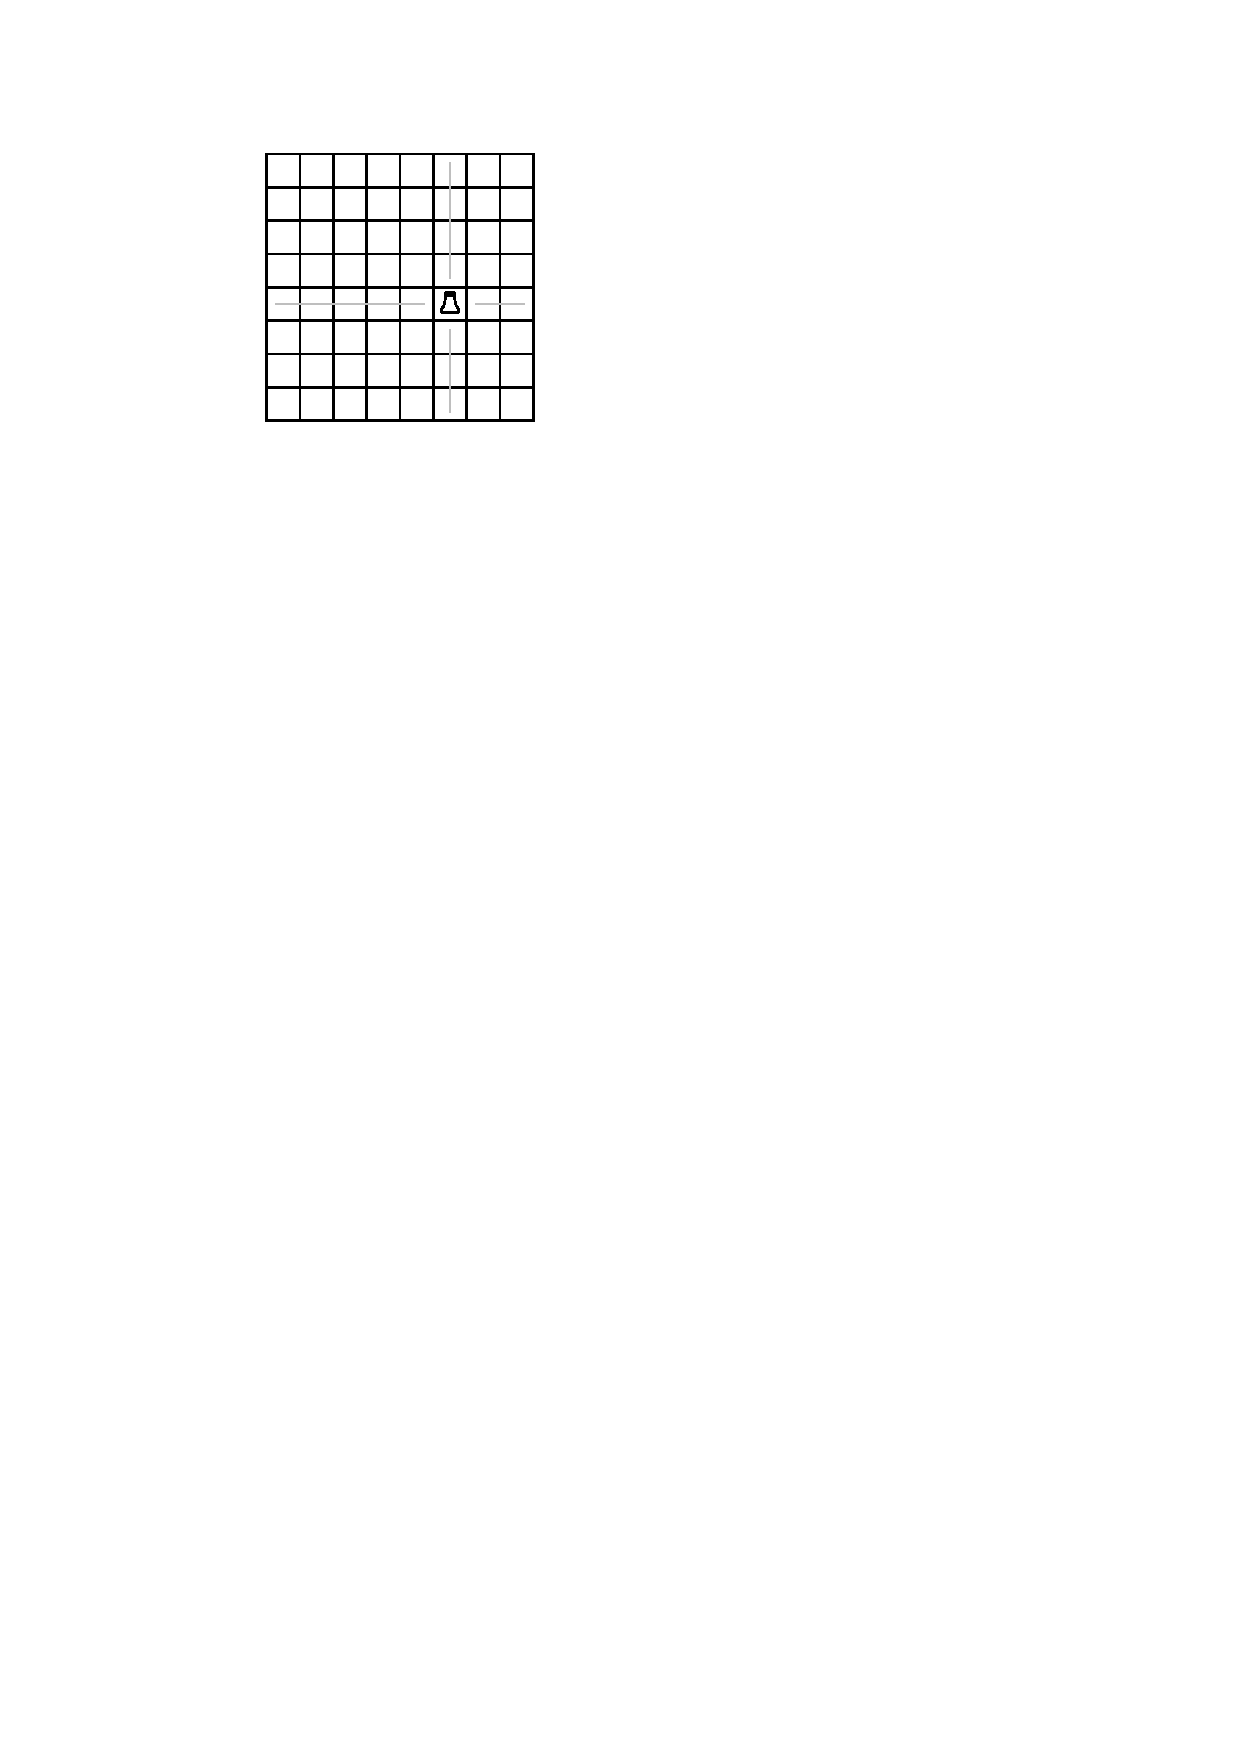
\includegraphics[page=1]{board}
    \end{center}

    \bparts
    \ppart{4}
        How many ways are there to place $n$ rooks on the board, such that no two rooks are in the same row or the same column? 

        \newpage
    \begin{center}
        \includegraphics[page=2]{board}
    \end{center}

        \ppart{8} Now suppose that the 2 squares on the diagonal in the top-left corner (as shown in gray) cannot be used.
        How many ways are there to place $n$ rooks so that no rook is placed on any of these gray squares, and again no two rooks are in the same row or column?

%        \remark{My intention was for this to be a somewhat hard problem. Is it?}

 %       \remark{This will be clearer with the picture: but the gray squares are those with coordinates $(1,1), (2,2)$ and $(3,3)$.}

        \eparts
\end{problem}

\newpage

\begin{problem}{10}
    Give a \textbf{combinatorial} proof of the identity
\[ \sum_{k=0}^n 2^k {n \choose k} = 3^n \]
for all positive integers $n$.

\emph{(You will get partial credit (up to a maximum of half the points) for a proof that is not a combinatorial proof).}
\end{problem}
\end{document}


